\documentclass[
  aps,
  prd,
  twocolumn,
  superscriptaddress,
  floatfix,
  nofootinbib,
  amsmath,
  amssymb
]{revtex4-2}

% ------------------------------------------------------------
% Standard packages
% ------------------------------------------------------------
\usepackage[T1]{fontenc}
\usepackage[utf8]{inputenc}
\usepackage{microtype}  % Better spacing
\usepackage{graphicx}   % Figures
\usepackage{dcolumn}    % Decimal-align tables
\usepackage{bm}         % Bold math
\usepackage{mathtools}  % Math extensions
\usepackage{physics}    % Bra-ket, derivatives, etc.
\usepackage{hyperref}   % Clickable refs
\usepackage{tikz}       % For diagrams if needed
\usetikzlibrary{matrix,positioning,arrows.meta}
\usepackage{float}
\usepackage{booktabs}   % Clean tables
\usepackage{xcolor}     % Colors for accents/notes
\usepackage{enumitem}   % Compact lists

% ------------------------------------------------------------
% Hyperref setup (APS compatible)
% ------------------------------------------------------------
\hypersetup{
  colorlinks=true,
  linkcolor=blue,
  citecolor=blue,
  urlcolor=blue,
  pdfauthor={Michael DeMasi},
  pdftitle={Primitive Integer Kernel of the Standard Model Decoupling Matrix}
}

% ------------------------------------------------------------
% Common macros
% ------------------------------------------------------------
\newcommand{\MSbar}{\overline{\text{MS}}}
\newcommand{\alphas}{\alpha_s}
\newcommand{\alphaEM}{\alpha}
\newcommand{\alphaTwo}{\alpha_2}

\newcommand{\ChiVec}{\chi = (16,13,2)}
\newcommand{\OmegaSM}{\Omega = \alphas^{16}\alphaTwo^{13}\alphaEM^{2}}

% Convenience macros
\newcommand{\MZ}{M_Z}
\newcommand{\GN}{G_N}
\newcommand{\mpl}{m_p}

% For SNF matrices
\newcommand{\DeltaW}{\Delta W}

% ------------------------------------------------------------
% Bibliography style (APS)
% ------------------------------------------------------------
\bibliographystyle{apsrev4-2}

% ------------------------------------------------------------
% Start of document
% ------------------------------------------------------------
\begin{document}

\title{Primitive Integer Kernel of the Standard Model Decoupling Matrix and Its Composite Gauge Coupling}

\author{Michael DeMasi}
\affiliation{Independent researcher, Milford, Connecticut 06460, USA}

\date{\today}

\begin{abstract}
The one--loop decoupling matrix of the Standard Model (SM) gauge sector is built entirely from fixed representation--theoretic integers. Using exact integer arithmetic, we compute its Smith normal form and find invariant factors $(1,8)$, implying a one--dimensional primitive integer right--kernel fixed solely by the SM field content. In the gauge--log basis this kernel becomes the unique integer triplet $\chi \equiv (16,13,2)$, which in turn defines the composite, parameter--free gauge coupling $\Omega \equiv \alpha_s^{16}\alpha_2^{13}\alpha^{2}$. Evaluated at $\mu=M_Z$ with PDG inputs in the $\MSbar$ scheme, $\Omega(M_Z)$ yields a closure ratio
$Z_G \equiv \alpha_G^{pp}/\Omega(M_Z) = 0.9143$ with the dimensionless proton--proton gravitational coupling $\alpha_G^{pp} = G_N m_p^2/(\hbar c)$. Treating $\alpha_s(M_Z)$ as unknown and enforcing $Z_G=1$ gives a leave--one--out closure value $\alpha_s^{*}(M_Z)=0.117341$, compatible with the current world average. No gravitational dynamics or model are assumed; the comparison is reported as a numerical observation. All steps are implemented with exact integer arithmetic and are fully reproducible via an accompanying open--source archive, which documents this previously unrecognized SM--internal integer invariant and its associated composite gauge coupling.
\end{abstract}


\maketitle



\section{Introduction}
The one--loop decoupling matrix of the Standard Model (SM) gauge
sector is fixed entirely by representation--theoretic integers%
~\cite{PeskinSchroeder1995_QFT,Langacker2009_RMP,Langacker2017_SMBeyond}.
As a result, any structural features it possesses are automatically
independent of renormalization scheme and gauge basis.  Viewed as an
integer matrix, it admits canonical invariants under all unimodular
transformations, and these encode basis--independent relations among
the gauge interactions%
~\cite{KannanBachem1979_SNF,Newman1997_SNF}.  Here we isolate this
purely arithmetic content by computing the Smith normal form (SNF) of
the SM one--loop decoupling matrix using standard polynomial--time
algorithms~\cite{KannanBachem1979_SNF}.

The SNF yields invariant factors $(1,8)$, demonstrating that the
integer right--kernel is one--dimensional and uniquely fixed by the SM
field content.  Transported to the gauge--log basis, this kernel takes
the primitive form
\begin{equation}
  \chi \equiv (16,13,2),
  \label{eq:chi}
\end{equation}
providing a basis--independent weighted direction in gauge--coupling space.

Exponentiating the associated projection defines the composite,
parameter--free quantity
\begin{equation}
  \Omega \equiv \alpha_s^{16}\,\alpha_2^{13}\,\alpha^{2},
\end{equation}
which depends solely on the SM gauge couplings and the integer data encoded in
$\chi$.  Using PDG inputs at $\mu = M_Z$~\cite{PDG2024}, the numerical value of
$\Omega$ lies close to the dimensionless proton--proton gravitational coupling
$\alpha_G^{pp} = G_N m_p^2 / (\hbar c)$ constructed from CODATA 2022
constants~\cite{CODATA2022_RMP}.  This proximity is reported strictly as a
numerical observation; no gravitational assumptions are introduced.

To test the internal consistency of this SM--derived structure, we perform a
leave--one--out (LOO) closure analysis in which $\alpha_s(M_Z)$ is treated as
unknown and determined by enforcing the unit--closure condition
\begin{equation}
  Z_G \equiv \frac{\alpha_G^{pp}}{\Omega(M_Z)} = 1,
  \label{eq:ClosureCond}
\end{equation}
while $\alpha_2(M_Z)$ and $\alpha(M_Z)$ are held at their PDG values.  This
procedure determines a specific closure value $\alpha_s^{*}(M_Z)$; future
precision determinations of the strong coupling that differ significantly from
$\alpha_s^{*}(M_Z)$ would falsify the closure relation.

The remainder of this Letter presents the integer SNF computation, constructs
the composite $\Omega$, evaluates its numerical value, and performs the LOO
test.  All results are fully reproducible through the accompanying Zenodo
archive~\cite{DeMasi_SM_Integer_Kernel_Certificate_2025}.

\section{Integer decoupling matrix and Smith normal form}
\label{sec:integer}

\subsection{Field content and one--loop weights}

The field content and quantum numbers follow the standard SM
assignments~\cite{PeskinSchroeder1995_QFT,Langacker2017_SMBeyond,PDG2024}.
To apply the Smith normal form to the one--loop decoupling matrix, we
construct an integerized weight matrix $W_{\mathbb Z}$ in which all
hypercharge contributions $w_1$ are rendered integral by a single overall
normalization of the $U(1)_Y$ weights.\footnote{%
The relative factors $12$ (fermions) and $3$ (scalars) arise from the
standard one--loop hypercharge coefficients---$4$ for Weyl fermions and
$1$ for scalar degrees of freedom---multiplied by the minimal global
integer normalization that makes all hypercharge weights in $W_{\mathbb Z}$
integral.  This overall scaling does not affect the primitive SNF kernel.}
Using the standard one--loop coefficients, the fermionic and scalar
contributions take the form
\begin{equation}
  w_{1}^{(f)} = 12\sum Y^{2}, 
  \qquad
  w_{1}^{(s)} = 3\sum Y^{2},
  \label{eq:w1integerized}
\end{equation}
ensuring that every entry of $W_{\mathbb Z}$ (and therefore of
$\Delta W_{\rm EM}$) is an integer.  The integer normalization of the
hypercharge column does not modify the primitive SNF kernel.
Table~\ref{T:Wcols} lists the light--species contributions entering
$W_{\mathbb Z}$ on a generic renormalization window~$W$.

\begin{table}[H]
\centering
\caption{Light species columns for $W_{\mathbb Z}$ on a window $W$.
Here $N_g$ denotes the number of fermion generations and $N_H$ the number of
Higgs doublets.  Hypercharge weights are made integral using
Eq.~\eqref{eq:w1integerized}.}
\label{T:Wcols}
\setlength{\tabcolsep}{1pt}
\renewcommand{\arraystretch}{1.08}
\begin{tabular}{lccccccc}
\hline
Species & $(SU(3),SU(2),Y)$ & dof$_{\rm spec}$ & $2T_3$ & $2T_2$ & $w_3$ & $w_2$ & $w_1$ \\
\hline
$Q_L$  & $(\mathbf 3,\mathbf 2,\,1/6)$   & $6N_g$ & 1 & 1 & $6N_g$ & $6N_g$ & $12\!\sum Y^2$ \\
$u_R$  & $(\mathbf 3,\mathbf 1,\,2/3)$   & $3N_g$ & 1 & 0 & $3N_g$ & $0$    & $12\!\sum Y^2$ \\
$d_R$  & $(\mathbf 3,\mathbf 1,\,-1/3)$  & $3N_g$ & 1 & 0 & $3N_g$ & $0$    & $12\!\sum Y^2$ \\
$L_L$  & $(\mathbf 1,\mathbf 2,\,-1/2)$  & $2N_g$ & 0 & 1 & $0$    & $2N_g$ & $12\!\sum Y^2$ \\
$e_R$  & $(\mathbf 1,\mathbf 1,\,-1)$    & $1N_g$ & 0 & 0 & $0$    & $0$    & $12\!\sum Y^2$ \\
$H$    & $(\mathbf 1,\mathbf 2,\,1/2)$   & $2N_H$ & 0 & 1 & $0$    & $2N_H$ & $3\!\sum Y^2$  \\
$W$    & adj.\ $(\mathbf 1,\mathbf 3,0)$ & $1$    & 0 & 4 & $0$    & 4      & 0 \\
$G$    & adj.\ $(\mathbf 8,\mathbf 1,0)$ & $1$    & 6 & 0 & 6      & 0      & 0 \\
\hline
\multicolumn{8}{l}{%
\parbox{\linewidth}{\footnotesize\textit{Note:}
For Weyl fermions $w_1^{(f)} = 12\sum Y^2$ and for scalar degrees of
freedom $w_1^{(s)} = 3\sum Y^2$.
For the Higgs doublet $H\!\sim(\mathbf 1,\mathbf 2,1/2)$ one has
$\sum_{\rm dof} Y^2 = \tfrac12$, giving $w_1(H)=3$.  All entries of
$W_{\mathbb Z}$ (and hence $\Delta W_{\rm EM}$) are therefore integral.}}
\end{tabular}
\end{table}

\subsection{Decoupling windows and the matrix \texorpdfstring{$\Delta W$}{ΔW}}

For any renormalization window $W=[\mu_{\rm low},\mu_{\rm high}]$, the one--loop
beta function of each gauge coupling receives contributions only from species
lighter than $\mu_{\rm high}$ and heavier than $\mu_{\rm low}$, consistent with
the standard decoupling of heavy fields~\cite{AppelquistCarazzone1975_Decoupling}.
The integerized weight matrix $W_{\mathbb Z}(W)$ therefore changes only when the
particle content of the window changes.  A \emph{decoupling step} $W\to W'$
induces a difference
\begin{equation}
  \Delta W = W_{\mathbb Z}(W') - W_{\mathbb Z}(W),
\end{equation}
which collects the integer weight jumps associated with that step.

For the electroweak--to--EM transition, the relevant $3\times 3$ block reduces
to a $2\times 3$ system after removing rows that are identical across the
window and hence contribute no change to Eq.~\eqref{eq:chi}.  Using the weights
in Table~\ref{T:Wcols}, this yields
\begin{equation}
  \Delta W_{\rm EM}
  =
  \begin{pmatrix}
    8 & 8 & 224 \\
    0 & 1 & 18
  \end{pmatrix},
  \label{eq:DeltaWEM}
\end{equation}
where the first row represents the net $SU(3)$, $SU(2)$, and integerized
$U(1)_Y$ weights of one SM generation, and the second captures the corresponding
Higgs and gauge--boson differences across the electroweak threshold.  No
tun\-able parameters enter this construction; it follows solely from the SM
field content.
\medskip
\paragraph*{Independence of window choice.}
The specific electroweak windows used to obtain
Eq.~\eqref{eq:DeltaWEM} are not unique.  Any other admissible
partition of the electroweak--to--EM transition, including splitting
the step $W\!\to\!W'$ into multiple subwindows with the same net light
particle content, corresponds to left--multiplying
$\Delta W_{\rm EM}$ by an element of ${\rm GL}(2,\mathbb Z)$ and
(possibly) adding or removing rows that are identical in both windows.
Because the Smith normal form and its primitive right--kernel are
invariant under such unimodular row operations, the invariant factors
$(1,8)$ and the generator $\chi_{\rm EM}=(-10,-18,1)$ are independent
of the particular window decomposition.

\subsection{Smith normal form and the primitive kernel}

To extract the integer structure of Eq.~\eqref{eq:DeltaWEM}, we compute its
Smith normal form (SNF),
\begin{equation}
  U\,\Delta W_{\rm EM}\,V
  = \mathrm{diag}(1,\,8,\,0),
  \label{eq:SNF}
\end{equation}
where $U\in{\rm GL}(2,\mathbb Z)$ and $V\in{\rm GL}(3,\mathbb Z)$ are unimodular
integer matrices.  The invariant factors $(1,8)$ show that
$\Delta W_{\rm EM}$ has integer rank~2 and therefore a
\emph{one--dimensional} primitive right--kernel over~$\mathbb Z$.

Solving $\Delta W_{\rm EM}\,\chi_{\rm EM}=0$ yields the primitive generator
\begin{equation}
  \chi_{\rm EM} = (-10,\,-18,\,1),
\end{equation}
unique up to overall sign.  Transporting this vector to the gauge--log basis
using the corresponding unimodular change of variables gives
\begin{equation*}
  \boxed{\chi \equiv (16,13,2)},
\end{equation*}
providing a basis--independent integer direction aligned with the one--loop
decoupling structure of the SM.

All SNF computations were performed with exact integer arithmetic using
standard algorithms~\cite{KannanBachem1979_SNF,Newman1997_SNF} and are fully
reproducible via the accompanying Zenodo archive%
~\cite{DeMasi_SM_Integer_Kernel_Certificate_2025}.

\begin{figure}[t]
\centering
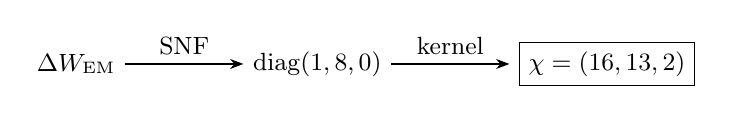
\begin{tikzpicture}[>=Stealth,node distance=1.5cm,every node/.style={font=\small}]
  \node (A) {$\Delta W_{\mathrm{EM}}$};
  \node[right=of A] (B) {$\mathrm{diag}(1,8,0)$};
  \node[right=of B] (C) {$\boxed{\chi=(16,13,2)}$};

  \draw[->] (A) -- node[above]{SNF} (B);
  \draw[->] (B) -- node[above]{kernel} (C);
\end{tikzpicture}
\caption{Smith normal form of $\Delta W_{\rm EM}$ yields invariant factors
$(1,8)$ and a unique primitive kernel $\chi=(16,13,2)$ (up to overall sign).}
\label{fig:integer-certificate}
\end{figure}
%---------------------------------------------------------------------------
\section{Gauge--log projection and the composite \texorpdfstring{$\Omega$}{Omega}}

Given the primitive kernel vector $\chi = (16,13,2)$ obtained in
Sec.~\ref{sec:integer}, we define the associated gauge--log projection
\begin{equation}
  \Xi = \chi \cdot \Psi
      = 16 \ln \alpha_s + 13 \ln \alpha_2 + 2 \ln \alpha,
  \label{eq:XiDef}
\end{equation}
where $\Psi = (\ln \alpha_s,\,\ln \alpha_2,\,\ln \alpha)$ collects the gauge
couplings in logarithmic form.  Because $\chi$ is integer--primitive and
basis--independent under all unimodular transformations, $\Xi$ represents the
unique SM--selected linear combination of gauge logs encoded in the one--loop
decoupling matrix.

Exponentiating Eq.~\eqref{eq:XiDef} yields the composite gauge coupling
\begin{equation}
  \Omega = e^{\Xi}
         = \alpha_s^{16}\,\alpha_2^{13}\,\alpha^{2},
  \label{eq:OmegaDef}
\end{equation}
which contains no tunable parameters and is fixed entirely by the SM gauge
representations.  The exponents coincide with the components of the primitive
kernel $\chi$, making $\Omega$ the unique weighted--power combination of the
gauge couplings dictated by the integer structure of $\Delta W_{\rm EM}$.

%---------------------------------------------------------------------------
\section{Numerical evaluation and closure ratio}
\label{sec:NumericalEvaluation}

We evaluate the composite $\Omega$ of Eq.~\eqref{eq:OmegaDef} at the electroweak
scale $\mu = M_Z$ using the 2024 PDG world averages for the SM gauge couplings
in the $\MSbar$ scheme~\cite{PDG2024}:
\begin{equation}
  \alpha_s(M_Z) = 0.1180, \quad
  \alpha_2(M_Z) = \frac{g_2^2}{4\pi}, \quad
  \alpha(M_Z)   = \frac{e^2}{4\pi}.
\end{equation}
Substituting these values into Eq.~\eqref{eq:OmegaDef} gives
\begin{equation}
  \Omega(M_Z)
    = \alpha_s^{16}(M_Z)\,\alpha_2^{13}(M_Z)\,\alpha^{2}(M_Z)
    = 6.46 \times 10^{-39},
  \label{eq:OmegaNumeric}
\end{equation}
in agreement with the fully reproducible computation archived in the accompanying
Zenodo repository~\cite{DeMasi_SM_Integer_Kernel_Certificate_2025}.

For comparison, we form the dimensionless proton--proton gravitational coupling
\begin{equation}
  \alpha_G^{pp}
    = \frac{G_N m_p^2}{\hbar c},
\end{equation}
using the CODATA 2022 recommended constants~\cite{CODATA2022_RMP}, which yields
\begin{equation}
  \alpha_G^{pp} = 5.91 \times 10^{-39}.
\end{equation}

Following the closure ratio convention, we define
\begin{equation}
  Z_G \equiv \frac{\alpha_G^{pp}}{\Omega(M_Z)},
\end{equation}
so that Eq.~\eqref{eq:ClosureCond} represents the closure condition.  Numerically,
\begin{equation}
  Z_G = 0.9143.
\end{equation}

No parameters are tuned in forming $\Omega$; its value is fixed entirely by SM
inputs and the integer kernel of Sec.~\ref{sec:integer}.  The proximity of $Z_G$ to unity
is a numerical observation only, and no gravitational model is assumed or invoked.

%---------------------------------------------------------------------------
\section{Leave--one--out closure for the strong coupling}

The composite $\Omega$ in Eq.~\eqref{eq:OmegaDef} depends on the three gauge
couplings evaluated at $\mu = M_Z$.  A natural leave--one--out (LOO) test is to
treat the strong coupling $\alpha_s(M_Z)$ as an unknown and impose the
\emph{closure} condition Eq.~\eqref{eq:ClosureCond} while keeping
$\alpha_2(M_Z)$ and $\alpha(M_Z)$ fixed to their PDG values~\cite{PDG2024}.
This determines a LOO value for the strong coupling,
\begin{equation}
  \alpha_s^{*}(M_Z)
  =
  \left[
    \frac{\alpha_G^{pp}}
         {\alpha_2^{13}(M_Z)\,\alpha^{2}(M_Z)}
  \right]^{1/16},
  \label{eq:alphasClosure}
\end{equation}
obtained directly from enforcing Eq.~\eqref{eq:ClosureCond}.

Using the same numerical inputs as in Sec.~\ref{sec:NumericalEvaluation}, we find
\begin{equation}
  \alpha_s^{*}(M_Z) = 0.117341,
\end{equation}
slightly below the PDG 2024 world average
$\alpha_s(M_Z) = 0.1180 \pm 0.0009$~\cite{PDG2024} and well within current
experimental uncertainties.  In this LOO interpretation, the SM--determined
composite $\Omega$ and the dimensionless quantity $\alpha_G^{pp}$ together
select a specific closure value for the strong coupling; future measurements of
$\alpha_s(M_Z)$ that differ significantly from $\alpha_s^{*}(M_Z)$ would
indicate a breakdown of the closure relation~\eqref{eq:ClosureCond}.

The integer kernel $\chi$ itself is unaffected by this procedure, as it is fixed
entirely by the SNF of $\Delta W_{\rm EM}$.  The LOO test acts only on the
numerical inputs and provides an experimentally accessible consistency check for
the SM--derived composite $\Omega$.

%---------------------------------------------------------------------------
\section{Conclusions}

We have examined the exact integer structure of the Standard Model
one--loop decoupling matrix and computed its Smith normal form.  The
resulting invariant factors $(1,8)$ imply a one--dimensional primitive
integer kernel fixed solely by the SM field content.  Transported to the
gauge--log basis, this kernel yields the triplet $\chi = (16,13,2)$,
which defines a unique SM--selected weighted--power combination of the
gauge couplings.

Exponentiating the associated projection produces the composite quantity
$\Omega = \alpha_s^{16}\alpha_2^{13}\alpha^{2}$, which contains no
tun\-able parameters and is determined entirely by the SM gauge
  representations.  Evaluated at $\mu = M_Z$ using PDG inputs, $\Omega$
numerically aligns with the dimensionless proton--proton gravitational
coupling at the level $Z_G = \alpha_G^{pp}/\Omega(M_Z) \simeq 0.9143$.
This comparison is purely numerical and does not invoke any
gravitational model.

A leave--one--out closure test, in which $\alpha_s(M_Z)$ is fixed by
demanding $Z_G = 1$, yields $\alpha_s^{*}(M_Z) = 0.117341$, well within
the current PDG world--average band.  In this interpretation, the
SM--determined composite $\Omega$ and the measured quantity
$\alpha_G^{pp}$ single out a specific closure value of the strong
coupling; future determinations of $\alpha_s(M_Z)$ that deviate
significantly from $\alpha_s^{*}(M_Z)$ would indicate a breakdown of the
closure relation.

All calculations are performed with exact integer arithmetic and are
fully reproducible using the accompanying Zenodo archive.  These results
identify a previously unrecognized SM--internal integer invariant and
its associated composite coupling, illustrating how exact--integer
methods can expose robust, scheme--independent structure in
renormalization--group decoupling matrices.



\appendix
\section*{Appendix: Reproducibility Package}

This repository provides an exact and fully reproducible computation of:
\begin{enumerate}
\item the Smith normal form (SNF) of the Standard Model one--loop decoupling matrix 
      \(\Delta W_{\mathrm{EM}}\),
\item the primitive integer kernel 
      \(\chi_{\mathrm{EM}} = (-10,-18,1)\),
\item its unimodular transport to the gauge--log basis 
      \(\chi = (16,13,2)\),
\item the Standard Model couplings 
      \(\alpha(M_Z)\), \(\alpha_2(M_Z)\), \(\alpha_s(M_Z)\),
\item the composite quantity 
      \(\Omega = \alpha_s^{16}\alpha_2^{13}\alpha^{2}\),
\item the dimensionless proton--proton gravitational coupling 
      \(\alpha_G^{pp}=G_N m_p^2/(\hbar c)\),
\item the closure ratio 
      \(Z_G = \alpha_G^{pp}/\Omega\)  
      and its inverse \(Z_G^{-1}=\Omega/\alpha_G^{pp}\),
\item the leave--one--out strong coupling \(\alpha_s^{\star}(M_Z)\).
\end{enumerate}

All integer algebra is performed with exact arithmetic, and all numerical
quantities are computed directly from \texttt{pins.json}.  
No geometric modeling or additional assumptions are used%
~\cite{DeMasi_SM_Integer_Kernel_Certificate_2025}.

\subsection*{Repository Contents}

\begin{verbatim}
sm_integer_kernel_certifier.py   
    # Main reproducibility script

pins.json                        
    # SM and SI input constants

results.json                     
    # Auto-generated machine-readable output

stdout.txt                       
    # Auto-generated readable summary
\end{verbatim}

\subsection*{How to Run}

Requires Python $\ge$ 3.8 and SymPy $\ge$ 1.9:
\begin{verbatim}
    python3 sm_integer_kernel_certifier.py
\end{verbatim}
\medskip
\subsection*{Matrix Definition}

\begin{equation*}
\Delta W_{\mathrm{EM}} =
\begin{pmatrix}
  8 & 8 & 224 \\[2pt]
  0 & 1 & 18
\end{pmatrix}.
\end{equation*}

\medskip
\subsection*{Expected Output}

\begin{verbatim}
SNF invariant factors: [1, 8]
Primitive kernel in (SU3,SU2,EM): (-10, -18, 1)
Transported kernel ...            (16, 13, 2)

alpha(MZ)      = 0.007815248
alpha2(MZ)     = 0.033789820
alpha_s(MZ)    = 0.118000000
Omega          = 6.459725598437e-39
alphaG_pp      = 5.906149417424e-39
Z_G            = 0.91430345
Z_G^-1         = 1.09372878
alpha_s* (LOO) = 0.117341100
\end{verbatim}

If used academically, please cite the Zenodo DOI associated with this repository.



\bibliographystyle{apsrev4-2}
\bibliography{geo_cqg_refs}



\end{document}